\subsection{Architekturdiagramm }

Im dritten Kapitel wurden alle benötigten Dienste ausgewählt und ihre Notwendigkeit erläutert.
Nun muss aus allen Komponenten eine zusammenhängende Architektur aufgebaut werden.
Das folgende Diagramm soll die Verbindung zwischen allen Diensten aufzeigen:

\begin{figure}[htbp]
    \centering
    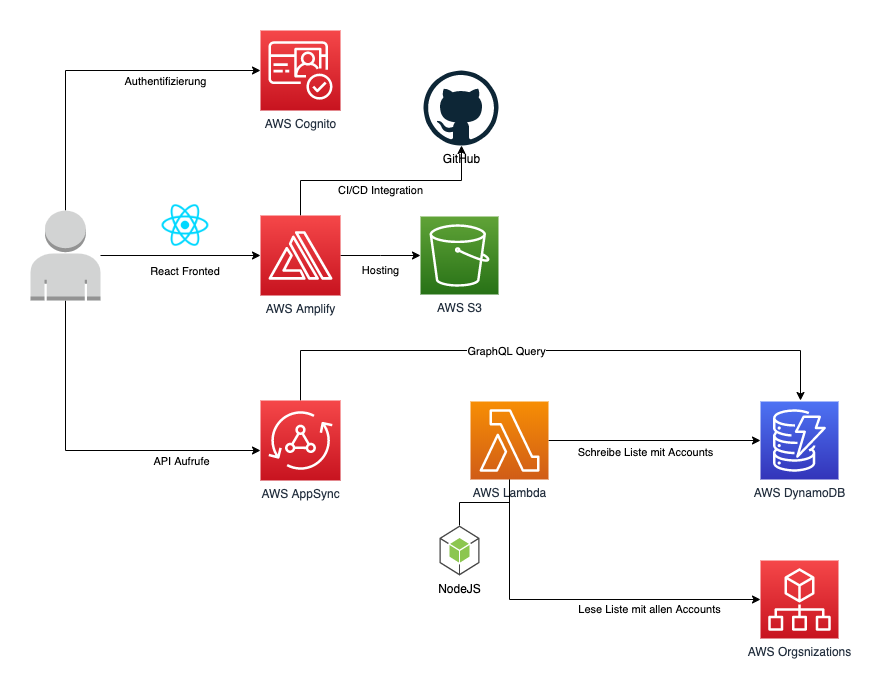
\includegraphics[width=1.0\textwidth]{50-Implementierung/Architektur.png}
    \caption{Übersicht der Architektur}
    \label{fig:meine-grafik}
\end{figure}

Das Diagramm zeigt die Kommunikationswege zwischen allen Diensten.
Sobald Anwender die Webanwendung aufrufen, kommunizieren sie mit den Diensten Cognito, Amplify Hosting sowie AppSync.
Das Frontend greift mithilfe von AppSync wiederrum auf die DynamoDB-Tabelle zu, um die benötigten Daten abzufragen.
Die Lambda-Funktion sorgt im Hintergrund dafür, dass die Daten in der Tabelle stets aktuell sind.
Dafür wird ein Zugriff auf einen anderen AWS Account benötigt.
GitHub wird für eine CI/CD Pipeline genutzt, und kann über Amplify konfiguriert werden.

Die Umsetzung der Anwendung erfolgt in fünf einzelnen Schritten.
Erzeugt werden alle Dienste über die Amplify CLI.
Zuerst müssen alle Voraussetzungen erfüllt werden.
Zu den Voraussetzungen zählt das Installieren aller benötigten Pakete und der Auswahl eines AWS Accounts.
Außerdem wird ein neues React-Projekt erstellt und Amplify initialisiert.
Im zweiten Schritt wird die GraphQL API über Amplify bereitgestellt.
Wie bereits in \textit{\ref{GraphQLResolver} \nameref{GraphQLResolver}} erwähnt kümmert sich AppSync gleichzeitig um den DynamoDB-Resolver und übernimmt so die Aufgabe eine DynamoDB-Tabelle anzulegen.
Während des dritten Schritts wird die Lambda-Funktion erstellt, welche die Backend-Logik abbildet.
Ein Lambda-Resolver wird im Rahmen der Bachelorarbeit nicht benötigt, da die Lambda-Funktion in einem regelmäßigen Zyklus ausgeführt wird.
Der vierte Schritt hat das Ziel eine Authentifizierung mit Cognito bereitzustellen.
Es muss sichergestellt werden, dass die Erstellung neuer Benutzeraccounts eingeschränkt wird.

Zum Testen wird eine lokale Umgebung verwendet, sodass der Code erst nach Fertigstellung hochgeladen wird, und die Anwendung zuvor nicht aufgerufen werden kann.
Das erlaubt ein schnelleres Testen sowie die Sicherheit, dass während der Entwicklung keine Daten öffentlich zugänglich sind.
Im letzten Schritt kann die lokale Anwendung, sofern sie ordnungsgemäß funktioniert, bei AWS gehosted werden, sodass sie über das Internet zugänglich ist.


In den folgenden Abschnitten werden alle einzelnen Schritte im Detail erläutert sowie auf potenzielle Probleme bei der Umsetzung hingewiesen.

\subsection{AWS Accountstruktur }
\label{Accountstruktur}

Zuerst ist es wichtig die Organisationsstruktur der AWS Accounts innerhalb der Mediengruppe RTL zu verstehen.
Zum einem ist es notwendig, da entschieden werden muss in welchem AWS Account die Webanwendung umgesetzt wird.
Zum anderen benötigt die Lambda-Funktion ebenfalls Zugriff auf den Dienst AWS Organizations.

Wie bereits in der Einleitung erwähnt besitzt die Mediengruppe RTL über 150 AWS Accounts.
Dafür gibt es mehrere Gründe.
Eine potenzielle Sicherheitslücke eines Accounts hat keinen Einfluss auf einen anderen Account, da alle Ressourcen voneinander isoliert sind.
Zusätzlich ist eine Kostenzuweisung deutlich einfacher, da pro Account eine eigene Kostenstelle angegeben werden kann.

Pro Funktion bzw. Projekt wird jeweils ein Account erstellt.
Aus Sicherheitsgründen wird zudem immer eine separate Umgebung für Test- und Produktivzwecke erzeugt.
Dadurch ist es möglich den Zugriff für bestimmte Umgebungen einzuschränken.
Eine Produktivumgebung sollte so wenig Zugriff wie möglich erlauben.
Beispiele für solche Accounts sind etwa \verb+Ntv-Streaming-Dev+ und \verb+Ntv-Streaming-Prod+.
Jeder der Accounts ist grundsätzlich unabhängig und weißt nur über die gemeinsame Organization eine Verbindung auf.
Zusätzlich gibt es für N-TV noch weitere Accounts für andere Projektbereiche.
Die Accounts \verb+Ntv-Web-Dev+ und \verb+Ntv-Web-Prod+ werden von anderen Personen betreut werden.
Daneben ist es möglich, dass noch weitere Accounts oder Entwicklungsumgebungen benötigt werden, etwa eine \verb+PreProd+ Umgebung.

Wie bereits im Abschnitt \textit{\ref{LambdaEntscheidung} \nameref{LambdaEntscheidung}} erwähnt, werden alle Accounts zentral über den Dienst AWS Organizations erstellt.
Es wird Zugriff auf den Master-Account benötigt um Informationen zu allen Accounts zu erhalten.
Details zur Umsetzung befinden sich im Abschnitt \textit{\ref{AccountübergreifenderZugriff} \nameref{AccountübergreifenderZugriff}}.

Für die Abteilung Datacenter and Clouds wurden speziell Accounts zum Testen erstellt.
Der Account \verb+Cbc-Clouds-Sandbox+ eignet sich für eine erste Testumgebung daher optimal.
Wird die Anwendung in Zukunft produktiv genutzt, kann sie ohne viel Aufwand in einen anderen Account migriert werden.


\subsection{Amplify Voraussetzungen}

\subsubsection{Einrichtung Amplify CLI}
\label{EinrichtungAmplify}
Bevor mit der Amplify CLI gearbeitet werden kann, muss sichergestellt sein, dass alle benötigten Pakete installiert sind und ein Zugang zu dem AWS Account \verb+Cbc-Clouds-Sandbox+ existiert.
Für die Verwendung von Amplify müssen die Pakete \verb+Node.js+ (Version \verb+>+ 10.x), \verb+npm+\footnote{Npm steht für Node Package Manager und ist ein Paketmanager für NodeJS. Mithilfe von npm können weitere Pakete installiert werden.} (Version \verb+>+ 5.x) und \verb+git+ (Version \verb+>+ 2.14.1) installiert werden.
Mithilfe von \verb+npm+ kann im Anschluss mit folgendem Befehl \verb+npm install -g @aws-amplify/cli+ die Amplify-CLI installiert werden.

Um den Zugang auf den AWS Account \verb+Cbc-Clouds-Sandbox+ zu realisieren, muss ein AWS IAM-User mit Zugangsdaten angelegt werden.
Diesen Prozess kann Amplify übernehmen.
Die Konfiguration wird mit dem Befehl \spverb+amplify configure+ gestartet.
Es wird nach der gewünschten Region sowie Benutzernamen gefragt.
Anschließend öffnet sich ein neues Browserfenster und der Vorgang kann fortgesetzt werden.
In Browser wird das Erstellen des Benutzers mit passenden Berechtigungen bestätigt.
Die im Browser angezeigten IAM Zugangsschlüssel werden im Terminal eingegeben und der Vorgang ist abgeschlossen.\cite[]{ImpVoraus}

Hinweis: Der interne Name des Projektes lautet Amplify-Kumo.
Kumo ist die japanische Bezeichnung für \glqq Cloud\grqq.
\\

\begin{lstlisting}[basicstyle=\ttfamily\small, breaklines=true , frame = single, backgroundcolor=\color{flashwhite} ]
# amplify configure
Follow these steps to set up access to your AWS account:

Sign in to your AWS administrator account:
https://console.aws.amazon.com/
Press Enter to continue

Specify the AWS Region
? region:(*@ \textrm{eu-central-1} @*)
Specify the username of the new IAM user:
? user name:(*@ \textrm{ amplify-kumo} @*)
Complete the user creation using the AWS console
https://console.aws.amazon.com/iam/[...]

Press Enter to continue

Enter the access key of the newly created user:
? accessKeyId:   (*@ \textrm{********************} @*)
? secretAccessKey:  (*@ \textrm{********************} @*)

Successfully set up the new user.
\end{lstlisting}

\clearpage
\subsubsection{Einrichtung React Projekt}

Eine weitere Voraussetzungen für Amplify ist die Erstellung eines neuen React-Projektes.
Dafür bieten die Entwickler von React den Befehl \verb+npx create-react-app+ an, welcher eine fertige Entwicklungsumgebung aufsetzt.
Dabei werden Aspekte wie die Ordnerstruktur, benötigte JavaScript-Pakete oder auch die Konfiguration eines Webservers übernommen.\cite[]{ReactNew}
Nachdem das Projekt erstellt wurde, kann der Webserver unter der Adresse \verb+http://localhost:3000+ gestartet werden.
Eine Testseite von React wird angezeigt.
\\
\begin{lstlisting}[basicstyle=\ttfamily\small, breaklines=true , frame = single, backgroundcolor=\color{flashwhite} ]
npx create-react-app amplify-kumo
cd amplify-kumo
npm start
\end{lstlisting}


\subsubsection{Konfiguration Amplify}

Nachdem das React-Projekt erfolgreich erstellt wurde, kann Amplify konfiguriert werden.
Anschließend ist es möglich alle gewünschten Dienste hinzuzufügen.

Zur Konfiguration muss \verb+amplify init+ ausgeführt werden.
Als erstes werden allgemeine Informationen benötigt, wie der Projektname oder das gewünschte Javascript-Framework.
Die darauffolgenden Pfade und Befehle sind nicht geändert worden.
Des weiteren wird der, in \textit{\ref{EinrichtungAmplify} \nameref{EinrichtungAmplify}} erstellte, IAM-User angegeben.
Nach kurzer Zeit ist das Amplify Projekt bereits in der Cloud erstellt worden und verfügbar.

Wie im Code ersichtlich, benutzt Amplify den Dienst AWS Cloudformation, sodass die gesamte Konfiguration in einem Template festgehalten wird.
Mit AWS CloudFormation ist möglich Templates zur Modellierung und Bereitstellung von AWS-Ressourcen zu erstellen.
Die Templates unterstützen JSON und YAML.
Amplify übersetzt alle Befehle in ein Cloudformation Template und startet es.
Da die gesamte Konfiguration der Cloudformation-Templates von Amplify übernommen wird, spielt es im Rahmen der Bachelorarbeit eine untergeordnete Rolle.

Außerdem wird bei der Initialisierung ein S3 Bucket sowie IAM-Rollen erstellt.
Das Bucket dient als Speicher für alle Konfigurationen und Templates.
Die IAM-Rollen werden für die Authentifizierung von Amplify benötigt.
Auch für die Lambda-Funktion sind IAM-Rollen von großer Bedeutung.
Im Abschnitt \textit{\ref{AccountübergreifenderZugriff} \nameref{AccountübergreifenderZugriff}} wird das Thema IAM-Rollen im Detail erklärt.

Es wurden alle Voraussetzungen erfüllt und die einzelnen Dienste können dem Projekt hinzugefügt werden.

\clearpage

\begin{lstlisting}[basicstyle=\ttfamily\small, breaklines=true , frame = single, backgroundcolor=\color{flashwhite} ]
[143302S0:amplify-kumo] master # amplify init

Enter a name for the project:(*@ \textrm{amplifykumo} @*)
Enter a name for the environment:(*@ \textrm{dev} @*)
Choose your default editor:(*@ \textrm{Visual Studio Code} @*)
Choose the type of app that you're building:(*@ \textrm{javascript} @*)
Please tell us about your project
What javascript framework are you using:(*@ \textrm{react} @*)
Source Directory Path:(*@ \textrm{src} @*)
Distribution Directory Path: (*@ \textrm{build} @*)
Build Command:(*@ \textrm{npm run-script build} @*)
Start Command:(*@ \textrm{npm run-script start} @*)

Using default provider  awscloudformation
Do you want to use an AWS profile? (Y/n) Y
Please choose the profile you want to use:(*@ \textrm{amplify-kumo} @*)
Initializing project in the cloud...

[...]

CREATE_COMPLETE DeploymentBucket AWS::S3::Bucket
CREATE_COMPLETE UnauthRole       AWS::IAM::Role
CREATE_COMPLETE AuthRole         AWS::IAM::Role
Initializing project in the cloud...

CREATE_COMPLETE amplify-kumo AWS::CloudFormation::Stack
Successfully created initial AWS cloud resources for
deployments.
Initialized provider successfully.
Initialized your environment successfully.

Your project has been successfully initialized and
connected to the cloud!

\end{lstlisting}


